\documentclass[final,hyperref={pdfpagelabels=false}]{beamer}
\usepackage{grffile}
\mode<presentation>{\usetheme{kaldi1}}
\usepackage[english]{babel}
\usepackage[latin1]{inputenc}
\usepackage{amsmath,amsthm, amssymb, latexsym, listings}
%\usepackage{times}\usefonttheme{professionalfonts}  % obsolete
%\usefonttheme[onlymath]{serif}
\boldmath
\usepackage[orientation=landscape,size=a0,scale=1.4,debug]{beamerposter}
% change list indention level
% \setdefaultleftmargin{3em}{}{}{}{}{}


%\usepackage{snapshot} % will write a .dep file with all dependencies, allows for easy bundling

\usepackage{array,booktabs,tabularx}
\newcolumntype{Z}{>{\centering\arraybackslash}X} % centered tabularx columns
\newcommand{\pphantom}{\textcolor{kaldiblack}} % phantom introduces a vertical space in p formatted table columns??!!

\listfiles

%%%%%%%%%%%%%%%%%%%%%%%%%%%%%%%%%%%%%%%%%%%%%%%%%%%%%%%%%%%%%%%%%%%%%%%%%%%%%%%%%%%%%%
\graphicspath{{figures/}}
 
\title{\huge The Kaldi Speech Recognition Toolkit}
\author{{Daniel Povey}$^1$, {Arnab Ghoshal}$^{2,3}$,
  {Gilles Boulianne}$^4$, {Luk\'{a}\v{s} Burget}$^{5,6}$, {Ond\v{r}ej 
    Glembek}$^5$, {Nagendra Goel}$^6$, \\
  {Mirko Hannemann}$^5$, 
  {Petr Motl\'{i}\v{c}ek}$^8$, {Yanmin Qian}$^9$, {Petr Schwarz}$^5$, 
  {Jan Silovsk\'{y}}$^{10}$, {Georg Stemmer}$^{11}$, {Karel Vesel\'{y}}$^5$}
\institute[]{   $^1$\,Microsoft Research, USA;
   $^2$\,University of Edinburgh, UK;
   $^3$\,Saarland University, Germany;
   $^4$\,Centre de Recherche Informatique de Montr\'{e}al, Canada; 
   $^5$\,Brno University of Technology, Czech Republic;
   $^6$\,SRI International, USA;
   $^7$\,Go-Vivace Inc., USA; $^8$\,IDIAP Research Institute, Switzerland; 
   $^9$\,Tsinghua University, China;
   $^{10}$\,Technical University of Liberec, Czech Republic; 
   $^{11}$\,University of Erlangen-Nuremberg, Germany
}
\date[]{}

%%%%%%%%%%%%%%%%%%%%%%%%%%%%%%%%%%%%%%%%%%%%%%%%%%%%%%%%%%%%%%%%%%%%%%%%%%%%%%%%%%%%%%
\newlength{\columnheight}
\setlength{\columnheight}{65cm}


%%%%%%%%%%%%%%%%%%%%%%%%%%%%%%%%%%%%%%%%%%%%%%%%%%%%%%%%%%%%%%%%%%%%%%%%%%%%%%%%%%%%%%
\begin{document}
\begin{frame}[fragile]
  \begin{columns}
    % ---------------------------------------------------------%
    % Set up a column 
    \begin{column}{.33\textwidth}
      \begin{beamercolorbox}[center,wd=\textwidth]{postercolumn}
        \begin{minipage}[T]{.95\textwidth}  % tweaks the width, makes a new \textwidth
          \parbox[t][\columnheight]{\textwidth}{ % must be some better way to set the the height, width and textwidth simultaneously
            % Since all columns are the same length, it is all nice and tidy.  You have to get the height empirically
            % ---------------------------------------------------------%
            % fill each column with content            

            \begin{block}{Problem Statement}
              \begin{itemize}
              \item You are a researcher who wants to try out a new method.
              \item You want other people to use your idea, if it works.
              \item You find that older toolkits (HTK, CMUSphinx) are too hard to modify.
              \item Also their license may not allow you to release your changes (HTK).
              \end{itemize}
            \end{block}
            \vfill
            \begin{block}{The Kaldi project}
              \begin{itemize}
              \item Open-source speech recognition toolkit, Apache-licensed.
              \item Began at 2009 Johns Hopkins University CLSP summer workshop.
              \item Further development included 2 summer workshops in Brno, Czech Republic, and ongoing work by the participants.
              \item Uses OpenFst code for decoding graph construction.
              \item Uses the BLAS and LAPACK libraries for linear algebra.
              \item Our closest competitor is probably the RWTH Aachen toolkit.
              \end{itemize}
            \end{block}
            \vfill
            \begin{block}{Our vision}
              \begin{itemize}
              \item Distributed community of users and contributors.
                \begin{itemize}
                \item Not a free-for-all; original authors moderate contributions.
                \item The Apache license allows you to fork the project.
                \end{itemize}
              \item Complete state-of-the-art recipes that run from public data
                \begin{itemize}
                \item These already exist for Resource Management and Wall Street Journal
                \item Switchboard recipe exists but is not yet state-of-the-art.
                \end{itemize}
              \item Code that's well structured and simple to understand.
              \item Thorough testing and documentation.
              \end{itemize}
            \end{block}
            \vfill
            \begin{block}{The structure of Kaldi}
              \begin{columns}
                \begin{column}{.44\textwidth}
              \begin{itemize}
              \item OpenFst for FST functions
              \item BLAS/LAPACK for linear algebra
              \item Core functions in C++
              \item Many simple command-line utilities
              \item Example shell scripts
              \end{itemize}
                \end{column}
                \begin{column}{.55\textwidth}
                  \centering
                  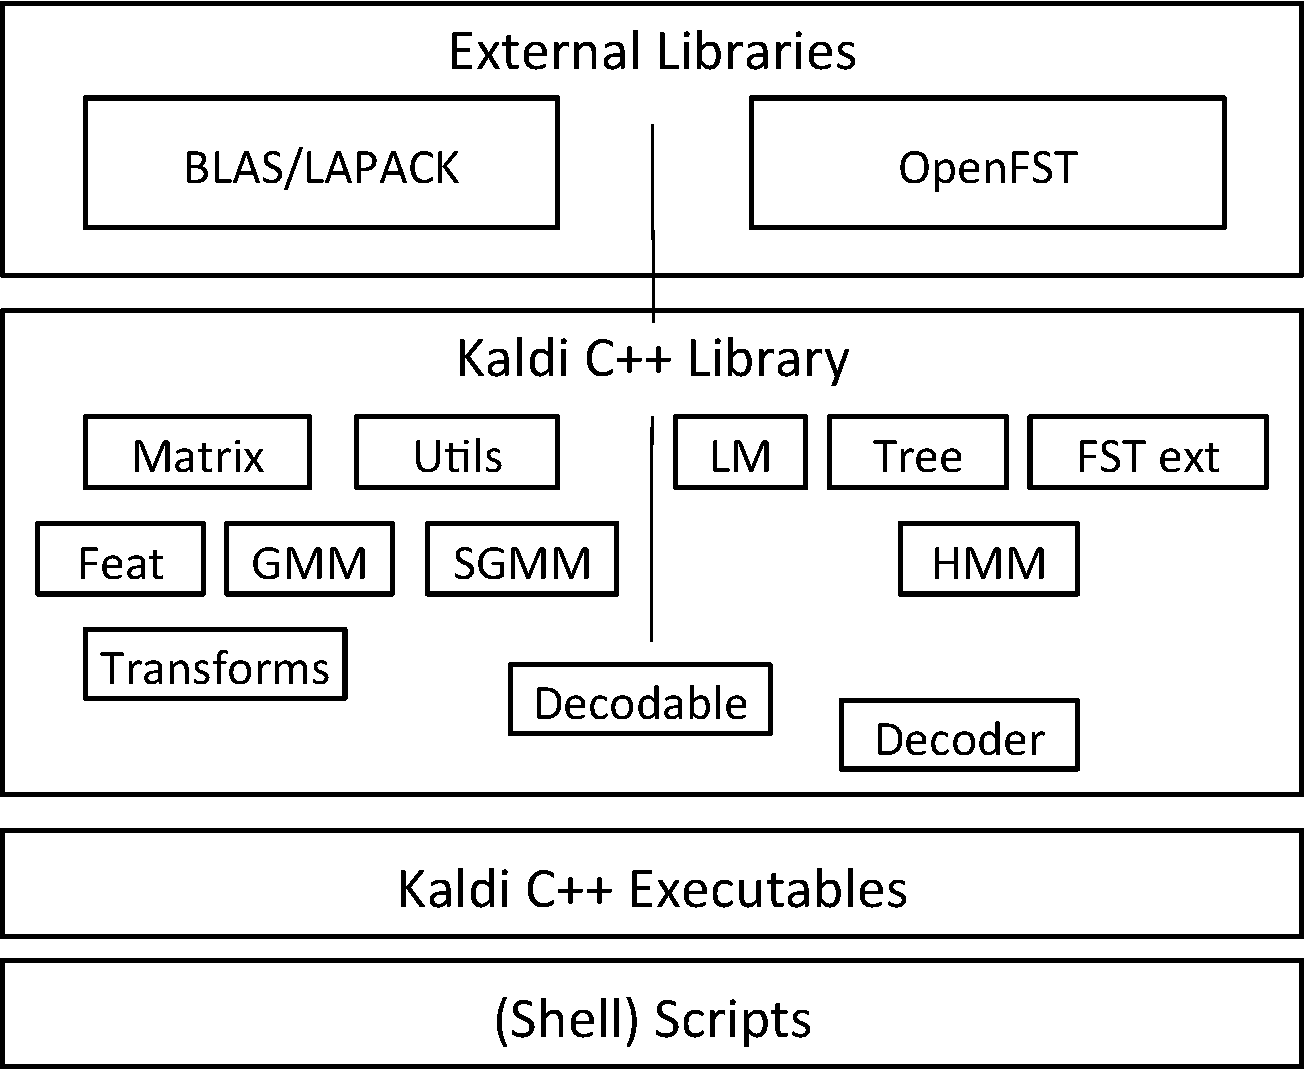
\includegraphics[width=0.99\linewidth]{figures/kaldi-lib.pdf} \vspace*{0.3in}
                \end{column}
              \end{columns}
              \vskip-1ex
            \end{block}
            \vfill
          }
        \end{minipage}
      \end{beamercolorbox}
    \end{column}
    % ---------------------------------------------------------%
    % end the column

    % ---------------------------------------------------------%
    % Set up a column 
    \begin{column}{.33\textwidth}
      \begin{beamercolorbox}[center,wd=\textwidth]{postercolumn}
        \begin{minipage}[T]{.95\textwidth} % tweaks the width, makes a new \textwidth
          \parbox[t][\columnheight]{\textwidth}{ % must be some better way to set the the height, width and textwidth simultaneously
            % Since all columns are the same length, it is all nice and tidy.  You have to get the height empirically
            % ---------------------------------------------------------%
            % fill each column with content
            

            \begin{block}{Example of Kaldi code}
              %% We couldn't get verbatim to work in here, so used a temporary tex file.
                  \includegraphics[width=0.9\linewidth,bb=128 517 486 725]{code-samples.pdf} 
            \end{block}
            \vfill
            \begin{block}{Acoustic modeling techniques supported in Kaldi}
              \begin{itemize}
              \item Acoustic front-end supports MFCC and PLP features, with 
                cepstral mean and variance normalization, LDA, STC/MLLT, HLDA,
                VTLN, etc.
              \item HMM/GMM acoustic models; phonetic decision trees.
              \item Also SGMMs, exponential transform.
              \item No language modeling code, but support converting ARPA 
                format LMs to FSTSs.
              \item WFST-based decoders, lattice generation.
              \item Discriminative training with MMI, boosted MMI (fMPE unfinished).
              \end{itemize}
            \end{block}
            \vfill
            \begin{block}{Example of top-level system building script}
              %% We couldn't get verbatim to work in here, so used a temporary tex file.
                  \includegraphics[width=0.9\linewidth,bb=128 472 495 725]{script-toplevel.pdf} 
            \end{block}
          }
        \end{minipage}
      \end{beamercolorbox}
    \end{column}
    % ---------------------------------------------------------%
    % end the column

    % ---------------------------------------------------------%
    % Set up a column 
    \begin{column}{.33\textwidth}
      \begin{beamercolorbox}[center,wd=\textwidth]{postercolumn}
        \begin{minipage}[T]{.95\textwidth} % tweaks the width, makes a new \textwidth
          \parbox[t][\columnheight]{\textwidth}{ % must be some better way to set the the height, width and textwidth simultaneously
            % Since all columns are the same length, it is all nice and tidy.  You have to get the height empirically
            % ---------------------------------------------------------%
            % fill each column with content

            \begin{block}{Segment of triphone training sript}
              %% We couldn't get verbatim to work in here, so used a temporary tex file.
                  \includegraphics[width=0.95\linewidth,bb=134 284 552 713]{script-lowlevel.pdf} 
            \end{block}
            \vfill
            \begin{block}{Comparison with previously published results}
              \begin{columns}
                \begin{column}{.5\textwidth}
                  \begin{table}
                    \centering
                    \small
                    \begin{tabular}{l c c c c c} \toprule
                      & \multicolumn{5}{c}{    Test set  }   \\ \cmidrule(l){2-6}
                      &  Feb'89 &  Oct'89 & Feb'91 & Sep'92 & Avg   \\
                      \cmidrule(lr){2-2}   \cmidrule(lr){3-3}                               \cmidrule(lr){4-4}            \cmidrule(lr){5-5}         \cmidrule(l){6-6}  
                      HTK    &  2.77    &  4.02   &  3.30  &  6.29  &  4.10 \\
                      Kaldi  &  3.20    &  4.21   &  3.50  &  5.86  &  4.06 \\ 
                      \bottomrule
                    \end{tabular}            
                  \end{table}
                  \vskip1ex
                \end{column}
                \begin{column}{.5\textwidth}
                  \begin{table}
                    \small
                    \centering
                    \begin{tabular}{@{} l @{} c c@{}}
                      \toprule 
                      & \multicolumn{2}{c}{    Test set  }   \\ \cmidrule(l){2-3}
                      &  Nov'92      &    Nov'93  \\ 
                      \cmidrule(lr){2-2} \cmidrule(r){3-3}
                      Bell      &  11.9        &  15.4    \\
                      HTK (+GD)  &  11.1        &  14.5   \\ 
                      KALDI      &  11.8        &  15.0   \\ \bottomrule
                    \end{tabular}
                  \end{table}
                \end{column}
              \end{columns}
              \begin{itemize}
              \item These are not our best results: they just show that with similar system setups, we get similar results.
                \begin{itemize}
                \item WSJ results in table use bigram LM.
                \end{itemize}
              \item Current best RM result: 1.78\% 
                \begin{itemize}
                \item System combination: LDA+MLLT+SAT+MMI with LDA+MLLT+SAT+SGMM+fMLLR).
                \end{itemize}
              \item Current best WSJ result: 4.39\% on eval'92 open-vocabulary test set.
                \begin{itemize}
                \item Train on SI-284, LDA+MLLT+SAT+SGMM, extended vocabulary, 4-gram LM trained from supplied trainscripts.
                \end{itemize}
              \end{itemize}
            \end{block}
%%             \vfill
%%             \begin{block}{Other Results}
%%               \begin{itemize}
%%               \item AR-Face: 110 classes, 110 train (``one-shot'' training), 550 test
%%               \end{itemize}
%%               \vskip-0.5ex
%%               \begin{table}
%%                 \small
%%                 \centering
%%                 \begin{tabular}{l @{} c c c@{}} \toprule
%%                   & RM (Avg) & WSJ Nov'92 & WSJ Nov'93 \\
%%                   \cmidrule(lr){2-2} \cmidrule(lr){3-3} \cmidrule(r){4-4}
%%                   Triphone                    & 3.97     & 12.5       &  18.3   \\
%%                   \,\, + fMLLR                & 3.59     & 11.4       &  15.5   \\ 
%%                   \,\, + LVTLN                & 3.30     & 11.1       &  16.4   \\ 
%%                   Splice-9 + LDA + MLLT       & 3.88     & 12.2       &  17.7   \\ 
%%                   \,\, + SAT (fMLLR)          & 2.70     & 9.6        &  13.7   \\ 
%%                   \,\, + SGMM + spk-vecs      & 2.45     & 10.0       &  13.4   \\ 
%%                   \qquad + fMLLR              & 2.31     & 9.8        &  12.9   \\ 
%%                   \qquad + ET                 & 2.15     & 9.0        &  12.3   \\
%%                   \bottomrule
%%                 \end{tabular}
%%               \end{table}
%%             \end{block}
%%             \vfill
%%             \begin{block}{Conclusions}
%%               \begin{itemize}
%%               \item 
%%               \end{itemize}
%%             \end{block}
          }
          % ---------------------------------------------------------%
          % end the column
        \end{minipage}
      \end{beamercolorbox}
    \end{column}
    % ---------------------------------------------------------%
    % end the column
  \end{columns}
  \vskip1ex
  %\tiny\hfill\textcolor{ta2gray}{Created with \LaTeX \texttt{beamerposter}  \url{http://www-i6.informatik.rwth-aachen.de/~dreuw/latexbeamerposter.php}}
%  \tiny\hfill{Created with \LaTeX \texttt{beamerposter}  \url{http://www-i6.informatik.rwth-aachen.de/~dreuw/latexbeamerposter.php} \hskip1em}
\end{frame}
\end{document}


%%%%%%%%%%%%%%%%%%%%%%%%%%%%%%%%%%%%%%%%%%%%%%%%%%%%%%%%%%%%%%%%%%%%%%%%%%%%%%%%%%%%%%%%%%%%%%%%%%%%
%%% Local Variables: 
%%% mode: latex
%%% TeX-PDF-mode: t
%%% End:
